\section{Consistency of Common Concepts}
\label{chap:improvement:concpets}

\mnote{Alternative for consistency relations}
In \autoref{chap:introduction}, we have motivated that models describing the same system share an overlap of information that leads to dependencies or in particular redundancies between the models, which need to be kept consistent.
%Such dependencies need to be kept consistent to preserve a contradiction-free specification of the system.
We have made these dependencies explicit by means of consistency relations.
In the following, we discuss the alternative consideration of redundancies, as a special case of dependencies, by means of common concepts.
We therefore provide an introductory example to be extended throughout the following considerations, explain the idea of \emph{\commonalities} and discuss in which cases it can be reasonably applied.


\subsection{Introductory Example}

\mnote{Example metamodels}
We employ a running example from the case study introduced in \autoref{chap:foundations:case_studies} involving \gls{PCM}, \gls{UML} and Java.
Consistency relations comprise the common and mostly one-to-one mappings between \gls{UML} and Java, as well as the ones proposed by \textcite{langhammer2015a} to represent \gls{PCM} architecture models in Java code and also in \gls{UML} class models.

\begin{figure}
	\centering
	\newcommand{\vdistance}{7.5em}
\newcommand{\hdistance}{(18em+0.4*\difftoafiveimage)}
\newcommand{\classwidth}{5.5em}
\newcommand{\labeldistance}{0.2em}
\newcommand{\mmborder}{1.5em}


\begin{tikzpicture}

\pgfdeclarelayer{bg}
\pgfsetlayers{bg,main}


% METACLASSES

\umlclassvarwidth{java_class}{}{Class}{
name\\
}{\classwidth}  

\umlclassvarwidth[, below=\vdistance of java_class.center, anchor=center]{uml_class}{}{Class}{
name\\
}{\classwidth} 

\umlclassvarwidth[, below left=0.5*\vdistance and \hdistance of java_class.center, anchor=center]{pcm_component}{}{Component}{
name\\
}{\classwidth} 


% METAMODELS

\coordinate (java_label_coordinate) at ([yshift=\labeldistance]java_class.north);
\node[mmlabel, anchor=south] (java_label) at (java_label_coordinate) {Java};

\coordinate (uml_label_coordinate) at ([yshift=-\labeldistance]uml_class.south);
\node[mmlabel, anchor=north] (java_label) at (uml_label_coordinate) {\acrshort{UML}};

\coordinate (pcm_label_coordinate) at ([xshift=-7*\labeldistance]pcm_component.west);
\node[mmlabel, right=6*\labeldistance of pcm_label_coordinate, anchor=east] (pcm_label) {\acrshort{PCM}};

\begin{pgfonlayer}{bg}
    \node[mmbg, fit=(java_class)(java_label_coordinate), inner sep=\mmborder] (java) {};
    \node[mmbg, fit=(uml_class)(uml_label_coordinate), inner sep=\mmborder] (uml) {};
    \node[mmbg, fit=(pcm_component)(pcm_label_coordinate), inner sep=\mmborder] (pcm) {};
\end{pgfonlayer}


% CONSISTENCY RELATIONS

\draw[directed consistency relation] (pcm_component) |- node[pos=0, above left] {$\mathvariable{co}$} node[above, pos=0.65, align=center] {$\setted{\tupled{\mathvariable{co}, \mathvariable{cl}} \mid \mathvariable{cl.name} = \mathvariable{co.name} + "\mathvariable{Impl}"}$} node[pos=1, below left] {$\mathvariable{cl}$} (java_class);
\draw[consistency relation] (java_class) -- node[pos=0, below right] {$\mathvariable{jcl}$} node[left] {$\setted{\tupled{\mathvariable{jcl}, \mathvariable{ucl}} \mid \mathvariable{jcl.name} = \mathvariable{ucl.name}}$} node[pos=1, above right] {$\mathvariable{ucl}$} (uml_class);
\draw[directed consistency relation] (pcm_component) |- node[pos=0, below left] {$\mathvariable{co}$} node[below, pos=0.65, align=center] {$\setted{\tupled{\mathvariable{co}, \mathvariable{cl}} \mid \mathvariable{cl.name} = \mathvariable{co.name} + "\mathvariable{Impl}"}$} node[pos=1, above left] {$\mathvariable{cl}$} (uml_class);

\end{tikzpicture}

	\caption[Consistency relations for extracts of Java, \acrshort{UML} and \acrshort{PCM}]{Simple metamodel extracts for Java, \gls{UML} and \gls{PCM} and consistency relations between them. Adapted from~\owncite[Fig.~1]{klare2019models}.}
	\label{fig:improvement:running_example}
\end{figure}

\mnote{Example relations}
In the following, we start with limited subsets of the metamodels, namely the one-to-one mapping between components in \gls{PCM} and classes in Java, whereby each component is mapped to a class but not vice versa, as depicted in \autoref{fig:improvement:running_example}.
Consistency relations require the existence of a class in \gls{UML} and Java for each \gls{PCM} component having the component name with an \enquote{Impl} suffix by an according unidirectional consistency relation, and an equally-named \gls{UML} class for each Java class and vice versa.
We extend the example in the following sections to explain the introduced concepts.


\subsection{Explicit Commonalities}
\label{chap:improvement:concepts:explicit}

\mnote{Common concepts}
In the given example, classes are redundantly represented in Java and \gls{UML}.
This requires them to be kept consistent, for example, by means of an according consistency relation.
As an alternative, redundant classes in a Java and a \gls{UML} model can also be considered representations of a \emph{common concept}, more precisely the common concept of a class in general object-oriented design.
Thus, rather than expressing this redundancy implicitly by means of a consistency relation and a transformation that preserves consistency to it, we propose to make the common concept explicit in an according metamodel and descriptions of how this concept \emph{manifests} in Java and \gls{UML}.
Then, instead of saying that each \gls{UML} class should corresponding to a Java class and vice versa, we would say that classes in \gls{UML} and Java are both representations of the same concept of a class in object-oriented design.

\begin{figure}
    \centering
    \newcommand{\vdistance}{7.5em}
\newcommand{\hdistance}{15em}
\newcommand{\classwidth}{5.5em}
\newcommand{\labeldistance}{1.2em}
\newcommand{\labelshift}{0.3*\classwidth}
\newcommand{\mmborder}{1em}

\begin{tikzpicture}

\pgfdeclarelayer{bg}
\pgfsetlayers{bg,main}


% METACLASSES

\umlclassvarwidth{java_class}{}{Class}{
name\\
}{\classwidth}  

\umlclassvarwidth[, right=\hdistance of java_class.north, anchor=north]{uml_class}{}{Class}{
name\\
}{\classwidth} 

\umlclassvarwidth[, above right=\vdistance and 0.5*\hdistance of java_class.north, anchor=north]{oo_class}{}{Class\vphantom{p}}{
name\\
}{\classwidth} 


% METAMODELS

\coordinate (java_label_coordinate) at ([yshift=\labeldistance]java_class.north west);
\node[mmlabel, anchor=west] (java_label) at (java_label_coordinate) {Java};

\coordinate (uml_label_coordinate) at ([xshift=\labelshift,yshift=\labeldistance]uml_class.north);
\node[mmlabel, anchor=center] (java_label) at (uml_label_coordinate) {UML};

\coordinate (oo_label_coordinate) at ([yshift=\labeldistance]oo_class.north);
\node[mmlabel, anchor=center] (oo_label) at (oo_label_coordinate) {Object-oriented Design};

\begin{pgfonlayer}{bg}
    \node[mmbg, fit=(java_class)(java_label_coordinate), inner sep=\mmborder] (java) {};
    \node[mmbg, fit=(uml_class)(uml_label_coordinate), inner sep=\mmborder] (uml) {};
    \node[conceptmmbg, minimum width=11.5em, fit=(oo_class)(oo_label_coordinate), inner sep=\mmborder] (oo) {};
\end{pgfonlayer}


% CONSISTENCY RELATIONS

\draw[manifests relation] (oo_class) -- node[manifests relation, above, sloped] {\manifestslabel} (java_class);
\draw[manifests relation] (oo_class) -- node[manifests relation, above, sloped] {\manifestslabel} (uml_class);

\end{tikzpicture}

    \caption[One \commonality example for object-oriented design]{\Conceptmetamodel for object-oriented design with a \texttt{Class} \commonality and its relations to the \concretemetamodels \gls{UML} and Java. Adapted from~\owncite[Fig.~2]{klare2019models}.}
    \label{fig:improvement:one_commonality_example}
\end{figure}

\mnote{Concepts and their relations}
We denote the actual metamodels that developers instantiate and want to keep consistent as \emph{\concretemetamodels}, whereas we denote metamodels that describe the concepts that such \concretemetamodels have in common as \emph{\conceptmetamodels}.
\autoref{fig:improvement:one_commonality_example} depicts the \concretemetamodels \gls{UML} and Java with their representations of classes.
In addition, it contains a \conceptmetamodel for object-oriented design, which contains the common concept of a class, shared by \gls{UML} and Java.
We denote a single common concept, such as a class, as a \emph{\commonality}.
Further \commonalities in object-oriented design would be interfaces or methods.
In general, a \commonality can be considered a \metaclass with the specific semantics of describing the commonalities between elements of \concretemetamodels.
We say that an element in a \concretemetamodel such as classes in \gls{UML} and Java are a \emph{manifestation} of a common concept.
The relation of a \commonality to these manifestations is denoted by a manifestation (\emph{\manifestslabel}) relation.
In the given example, the relations would especially define that each class manifestation conforms to a common class concept having the same name and vice versa, as depicted in the consistency relations defined in \autoref{fig:improvement:running_example}.

\mnote{Specification effort}
In fact, these manifestation relations can be considered consistency relations that are preserved by ordinary transformations.
Thus, in a first place the representation of common concepts in terms of explicit \commonalities introduces further effort, because it requires the definition of one metamodel and two transformations instead of a single transformation relating the \metaclasses directly.
This drawback is, however, reduced by several benefits, which we discuss in \autoref{chap:improvement:benefits}, such as mitigating trade-offs between correctness and reusability as well as improving comprehensibility.
Finally, such a specification can even reduce effort due to better scalability when adding further \concretemetamodels to keep consistent.
For example, if another object-oriented language such as \cplusplus shall be kept consistent, no matter whether only with \gls{UML} or indeed even with Java, only the manifestation relation from \commonalities in the object-oriented design \conceptmetamodel to \cplusplus has to be added, potentially along with some extensions of the \conceptmetamodel for information shared between \cplusplus and \gls{UML} as well between \cplusplus and Java that was not already shared between Java and \gls{UML}.
This already reduces the effort in comparison to defining both relations between \cplusplus and \gls{UML}, as well as between \cplusplus and Java.

\begin{figure}
    \centering
    \newcommand{\distance}{5em}
\newcommand{\circlesize}{3.7em}
\newcommand{\imagesdistance}{3.5*\distance+0.3*\difftoafiveimage}

\begin{tikzpicture}[
    concrete font/.style={font=\footnotesize},
    concept font/.style={font=\small\bfseries},
    concept color/.style={conceptmmbg}
]

% CONCEPTS
\def\concepta{(0,0) circle (\circlesize)}
\def\conceptb{(\distance,0) circle (\circlesize)}
\def\conceptc{(0.5*\distance,\distance) circle (\circlesize)}

% Filling
\fill[schematic metamodel] \concepta;
\fill[schematic metamodel] \conceptb;
\fill[schematic metamodel] \conceptc;

% Filling
\begin{scope}
    \clip \conceptb;
    \fill[concept color] \concepta;
\end{scope}

\begin{scope}
    \clip \conceptc;
    \fill[concept color] \conceptb;
\end{scope}

\begin{scope}
    \clip \concepta;
    \fill[concept color] \conceptc;
\end{scope}

% Borders
\draw \concepta;
\draw \conceptb;
\draw \conceptc;


% SUM
\def\suma{(\imagesdistance,0) circle (\circlesize)}
\def\sumb{(\imagesdistance+\distance,0) circle (\circlesize)}
\def\sumc{(\imagesdistance+0.5*\distance,\distance) circle (\circlesize)}

% Filling
\fill[concept color] \suma;
\fill[concept color] \sumb;
\fill[concept color] \sumc;

% Borders
\tikzstyle{reverseclip}=[insert path={(-\circlesize-\pgflinewidth,-\circlesize-\pgflinewidth) --
  (0, \distance+\circlesize+\pgflinewidth) --
  (\imagesdistance+\distance+\circlesize+\pgflinewidth, \distance+\circlesize+\pgflinewidth) --
  (\imagesdistance+\distance+\circlesize+\pgflinewidth, -\circlesize-\pgflinewidth) --
  (-\circlesize-\pgflinewidth,-\circlesize-\pgflinewidth)}
]

\begin{scope}
    \begin{pgfinterruptboundingbox}
    \path [clip] \suma [reverseclip];
    \path [clip] \sumb [reverseclip];
    \end{pgfinterruptboundingbox}
    \draw \sumc;
\end{scope}

\begin{scope}
    \begin{pgfinterruptboundingbox}
    \path [clip] \sumb [reverseclip];
    \path [clip] \sumc [reverseclip];
    \end{pgfinterruptboundingbox}
    \draw \suma;
\end{scope}

\begin{scope}
    \begin{pgfinterruptboundingbox}
    \path [clip] \suma [reverseclip];
    \path [clip] \sumc [reverseclip];
    \end{pgfinterruptboundingbox}
    \draw \sumb;
\end{scope}


% LABELS
\node[concept font, anchor=south] at (\imagesdistance+0.5*\distance,\distance-\circlesize) {SUM};
\node[concrete font, anchor=center, align=center] at (-0.3*\circlesize,-0.1*\circlesize) {Concrete\\Metamodel};
\node[concrete font, anchor=center, align=center] at (0.5*\distance,\distance+0.2*\circlesize) {Concrete\\Metamodel};
\node[concrete font, anchor=center, align=center] at (\distance+0.3*\circlesize,-0.1*\circlesize) {Concrete\\Metamodel};
\node[concept font, anchor=west, align=center] at (0.5*\distance+1.1*\circlesize, \distance+0.2*\circlesize) (concept_mm_label) {Concept\\Metamodel(s)};

\draw (concept_mm_label) -- (\distance,0.8*\circlesize);

\end{tikzpicture}
    %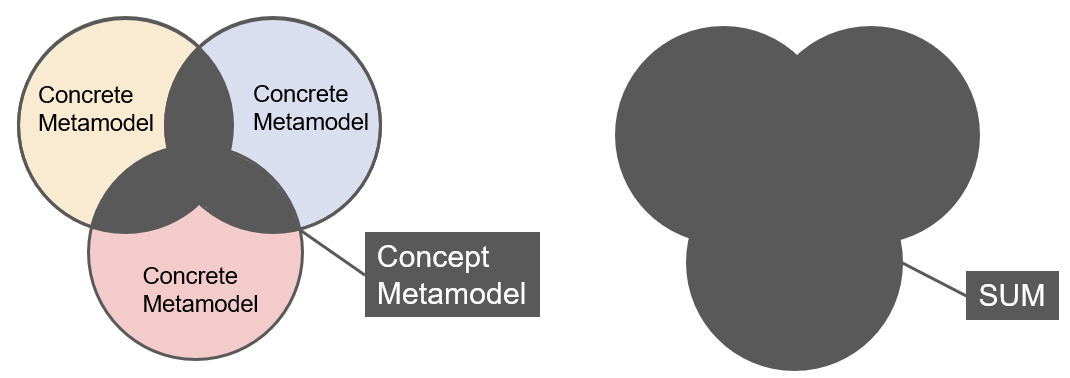
\includegraphics[width=\textwidth]{figures/quality/improvement/commonalities_and_sums.png}
    \caption[Commonalities compared to \acrlongpl{SUM}]{Sketched comparison for the scope of contents of \conceptmetamodels and \glspl{SUM}.}
    \label{fig:improvement:commonalities_and_sums}
\end{figure}

\mnote{Size of concept metamodels}
In general, a \conceptmetamodel has to contain \commonalities for all redundancies between the \concretemetamodels to keep consistent.
In a mathematical sense, this can be considered as the union of all pairwise intersections of the \concretemetamodels.
It can, however, not be precisely expressed as such, because elements may be similarly represented in the \concretemetamodels, but they are not the same.
One manifestation of the same \commonality may contain different information or encode it differently, such as using other units, than the others.
This already illustrates the essential difference to approaches in which one central model unifies all information about a system, called a \gls{SUM} (see \autoref{chap:foundations:multiview:osm}), from which the models used by different tools are derived by projections.
Such a \gls{SUM} can be seen as the union of all \concretemetamodels, whereas \concretemetamodels represent the union of their pairwise intersections, as illustrated in \autoref{fig:improvement:commonalities_and_sums}.


\subsection{Consistency Specification Types}
\label{chap:improvement:concepts:specification}

\mnote{Descriptive and normative specifications}
In \autoref{chap:networks:notions:normative_descriptive}, we have discussed the distinction of descriptive and normative specifications of consistency, which can be summarized as follows:
\begin{properdescription}
    \item[Descriptive Specification:] Descriptive specifications describe consistency relations that are \enquote{naturally} given when two metamodels represent common concepts redundantly or with common or dependent properties. 
    In that case, a notion of consistency already exists, formally or informally, to which the given specification must conform.
    This is, for example, the case for \gls{UML} class models and Java realizing object-oriented design.
    \item[Normative Specification:] Normative specifications prescribe consistency for metamodels for which no existing or common notion for consistency exists.
    This is especially the case if metamodels represent different abstractions or domains of a system, which have no implicit relations and for which different possibilities to relate them exist, such as an architecture description in \gls{PCM} and its implementation in Java.
\end{properdescription}
While descriptive consistency relations between two metamodels are usually definite, such as those for object-oriented design between \gls{UML} and Java, normative consistency relations may vary depending on the project context.
For example, several possible relations can be defined between an architecture description in \gls{PCM} and object-oriented design, such as the realization of each component as a class, as a bean in \glspl{EJB}, or as a complete project~\cite{langhammer2017a}.

\mnote{Suitability for descriptive specification}
Describing consistency by means of \commonalities and \conceptmetamodels especially promises to be useful for descriptive consistency specifications, where a \enquote{natural} relation exists due to elements representing common concepts.
It can, however, also be used to normatively define \commonalities in terms of a normative specification.
A component \commonality can, for example, define that a component manifests as a component in \gls{PCM} and as a class in \gls{UML} and Java, or, more generally, in an object-oriented design \conceptmetamodel.
This will, however, unlikely fit well for rather complex dependencies, such as a consistency relation requiring an implementation to fulfill some performance requirement.
In such a case, the complexity is in the specification of the relation anyway, which would have to be replicated when defining a \commonality between performance requirement and implementation.
Finally, this conforms to our distinction of structural and behavioral consistency relations given in \autoref{chap:networks:notions:types}, in which the \commonalities fit well for structural relations, on which we focus in this thesis anyway.

\mnote{Generalization}
In the following, we do not distinguish whether \commonalities are defined for common concepts that exist naturally, or for those which are prescribed by the definition of \conceptmetamodels and their \commonalities.
We will see that even for normative specifications \commonalities can be reasonably defined.
In \autoref{chap:improvement:application}, we also discuss how to combine ordinary transformations with the idea of \conceptmetamodels.

